\section{Prototype and Board Revisions}
\label{sec:hw-overview}

One V1.0 PCB was assembled for bring-up and the final tests. It measures \SI{202.77}{\milli\metre} by \SI{72.77}{\milli\metre} and has four 1~oz copper layers. The final resonant branch had two Wurth Elektronik 7443640470B inductors connected in series. The voltage-control firmware used for the final tests is described in Chapter~\ref{ch:control}.

Changes made during bring-up were recorded in V1.1. The timer-pin assignment and charge-pump-diode connection were corrected. Some component values and positions were also changed. No separate V1.1 board was manufactured. Differences between the drawings and fitted parts are noted so the tested configuration can be reproduced. Both complete schematic revisions are included in Appendix~\ref{app:hardware}.

\begin{table}[htbp]
\centering
\caption{Hardware used for the prototype tests.}
\label{tab:hardware-revision-status}
\begin{tabularx}{\textwidth}{@{}p{0.19\textwidth}p{0.31\textwidth}X@{}}
\toprule
Hardware & Build status & Use\\
\midrule
V1.0 board & Manufactured and tested, including bring-up modifications & Board shown in the photographs, layout, and measurements\\
Final resonant branch & Two \SI{4.7}{\micro\henry} resonant inductors in series & Used for the final tests\\
V1.1 schematic & Drawing revision; no separate test board & Documents the bring-up corrections\\
\bottomrule
\end{tabularx}
\end{table}

V2 continued this work with the MCU integrated on the converter board. The schematic and four-layer PCB layout are described in \cref{sec:hw-v2}. Preliminary powered V2 tests, including the leakage-only tank change and remaining input-bridge heating, are described in \cref{sec:res-v2-testing}. The earlier matched measurements were taken on the modified V1.0 board.

Before fabrication, the board passed the configured Altium design-rule check. During bring-up, insulation was checked at \SI{1000}{\volt} for \SI{30}{\second} with the available handheld tester. This was a laboratory check; standardized safety qualification requires a defined test procedure and conditions.

\begin{figure}[H]
\centering
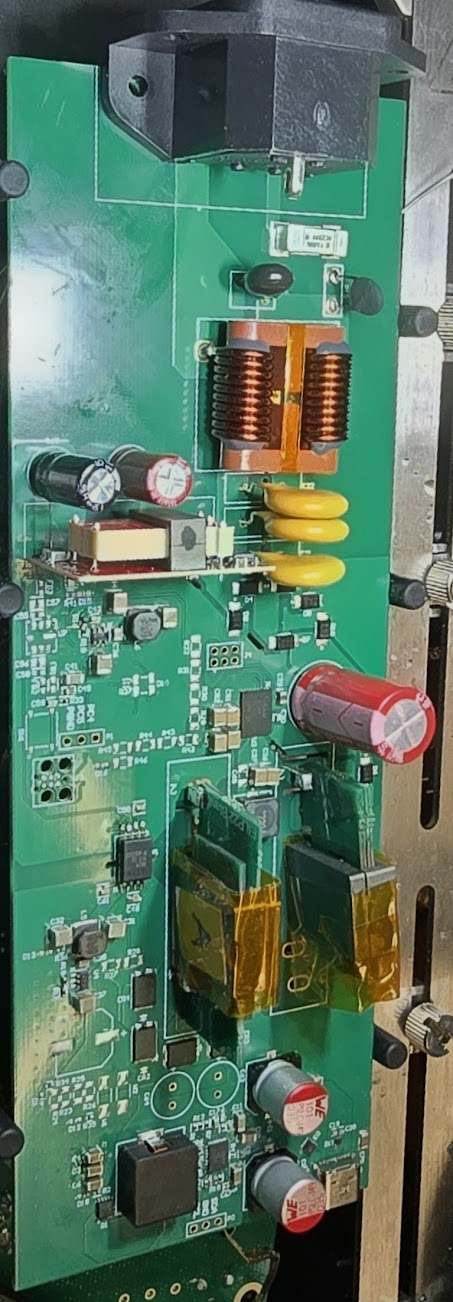
\includegraphics[angle=90,width=\linewidth]{Pictures/Thesis/07_Hardware/final_prototype_main_photo.png}
\caption{Assembled V1.0 prototype used for the final tests.}
\label{fig:final-prototype-main-photo}
\end{figure}
